
\documentclass{beamer}
\setbeamertemplate{navigation symbols}{}
    \addtobeamertemplate{frametitle}{\vspace*{-0.1cm}}{\vspace*{-0.5cm}}

\setbeamercolor{frametitle}{fg=black,bg=white}
\usepackage{tikz}
\usetikzlibrary{matrix}
\usepackage{dsfont}
\usetheme{CambridgeUS}
\usepackage[UKenglish]{babel}
\usepackage{graphicx}
\usepackage{fourier}


\begin{document}
\title[Hull-White model and calibration]{Hull-White Model and Calibration\\
Perfect Fit of the Term Structure}  



\date{\today} 
\author{M. Lobenwein, N. Weber, M. Pommer}



\begin{frame}
\titlepage
\end{frame} 


\begin{frame}
\frametitle[Table of Content]{Table of Content}
\vspace{0.4cm}
\tableofcontents
\end{frame} 

\AtBeginSection[]
{
\begin{frame}
\frametitle[Table of Content]{Table of Content}
\vspace{0.4cm}
\tableofcontents[currentsection]
\end{frame} 
}

\section{Introduction} 
\begin{frame}
\frametitle{Introduction} 
\begin{itemize}
\item Hull-White model: $dr_t = [\theta(t)-ar_t]dt + \sigma dW_t$
\item Since the Hull-White model is inhomogenous we can exactly fit the term structure
\item In order to achieve the perfect fit we construct a trinomial tree in two consecutive steps
\end{itemize}
\end{frame}


\section{Trinomial tree according to Hull} 
\begin{frame}
\frametitle{Trinomial tree according to Hull and White step one} 
\begin{block}{Options, Futures and other Derivatives by Hull and White}
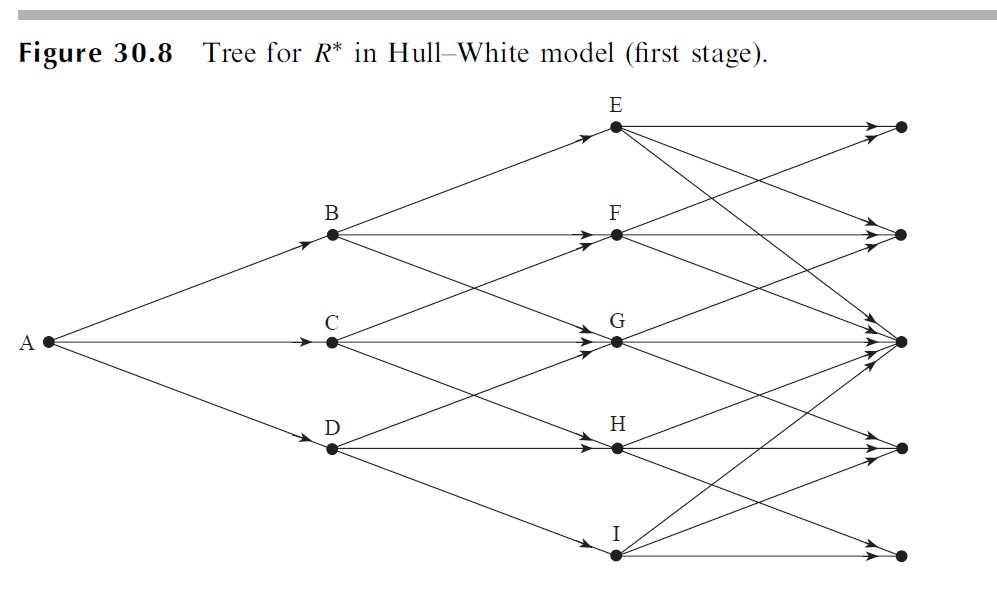
\includegraphics[width=0.7\textwidth]{Trinomialbaum hull White step one}
\end{block}
Dynamics: $dR^*_t = \sigma dW_t$, assuming $a=0$

\end{frame}


\begin{frame}
\frametitle{Trinomial tree according to Hull and White step two}
\begin{block}{Options, Futures and other Derivatives by Hull}
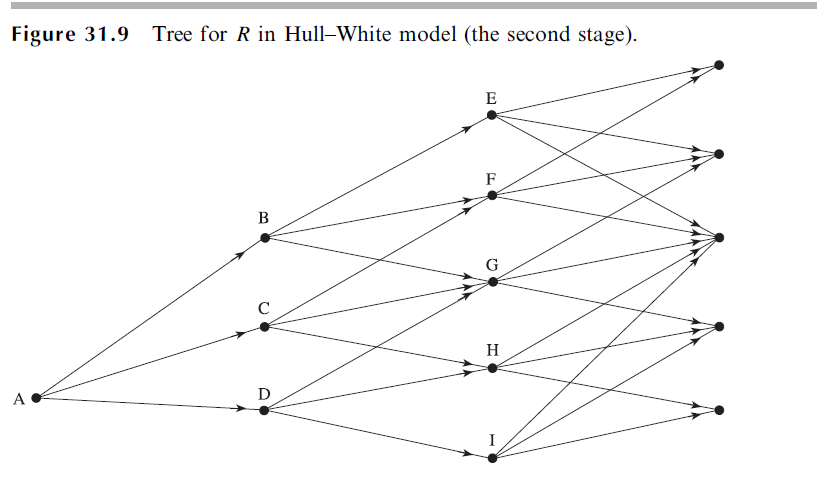
\includegraphics[width=0.7\textwidth]{Trinomialbaum hull White step two}
\end{block}
Dynamics: $dR_t = \theta(t)dt + \sigma dW_t$, assuming $a=0$

\end{frame}



\section{Calculations}

\subsection{Calculation of the probabilities}
\begin{frame}
\frametitle{Trinomial tree according to Hull and White step one} 
\begin{itemize}
\item During the first step the branching probabilities for going up, down and remaining constant are calculated
\item The difference $R^*(t+\Delta t) - R^*$ is normally distributed with mean $-aR^* \Delta t$ and variance $\sigma ^2 \Delta t$ 
\item We have to equate the theoretical mean and variance with the one in the model
\end{itemize}

\begin{align*}
p_u \Delta R-p_u \Delta R &= -aj\Delta R\Delta t\\
p_u\Delta R^2 + p_d \Delta R^2 &= \sigma ^2 \Delta t + a^2j^2 \Delta R^2 \Delta t^2\\
p_u + p_m + p_d &= 1
\end{align*}


\end{frame}






\begin{frame}
\frametitle{Trinomial tree according to Hull and White step one} 

This leads to the following probabilities:

\begin{align*}
p_u &= \frac{1}{6} + \frac{1}{2}(a^2j^2 \Delta t^2 - a j \Delta t)\\
p_m &= \frac{2}{3} + a^2j^2 \Delta t^2 \\
p_u &= \frac{1}{6} + \frac{1}{2}(a^2j^2 \Delta t^2 + a j \Delta t)\\
\end{align*}

\end{frame}



\subsection{Perfect fit of the term structure}
\begin{frame}
\frametitle{Trinomial tree according to Hull and White step two} 
\vspace{0.4cm}
We have to shift the nodes in order to fit the term structure
\begin{itemize}
\item We define $Q_{i,j}$ as the present value of a security that pays off 1 EUR at node $(i,j)$
\item We initialize $Q_{0,0} = 1$
\item We calcuate $\alpha_0$ such that the right price of the given zero coupond bond at time $\Delta t$ is perfectly met
\item Next we calculate the prices $Q_{1,j}$ at time 0 for all nodes $j$ as the multiplication of the respective probabilities and the zero coupond bonds according to $\alpha_0$
\item We can iteratively calculate all $\alpha_i$ and $Q_{i,j}$ to exactly fit the term structure with the following formulas
\end{itemize}

\vspace{-0.6cm}

\begin{align*}
\alpha_m &= \frac{ln \sum_{j=-n_m}^{n_m} Q_{m,j} e^{-j\Delta R \Delta t} - ln P_{m+1}}{\Delta t}\\
Q_{m+1,j} &= sum_k Q_{m,k}q(k,j) exp[-(\alpha_m + k \Delta R) \Delta t]
\end{align*}

\end{frame}



\section{Coding - Have Fun}

\begin{frame}
\frametitle{Trinomial tree according to Hull and White step two} 
We demonstrate how well the term structure is fit and how arbitrary cash flows and options on cash flows can be valued!\\

Have fun:)
\end{frame}







\end{document}